\documentclass[11pt, a4paper]{article}
\usepackage[space]{ctex}
\usepackage{amsmath}
\usepackage{tikz}
\usetikzlibrary{arrows,automata,positioning}
\usepackage{pgflibraryarrows}
\usepackage{pgflibrarysnakes}
\begin{document}
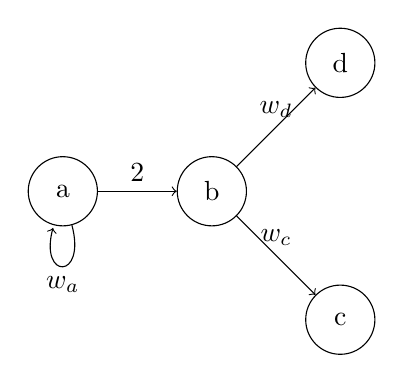
\begin{tikzpicture}
\node[state] (0){a};
\node[state] (1)[right=of 0]{b};
\node[state] (2)[below right=of 1]{c};
\node[state] (3)[above right=of 1]{d};
\path[->] (0) edge [loop below] node {$w_a$} (0)
		(0) edge node [above] {2} (1)
		(1) edge node [above] {$w_c$} (2)
		(1) edge node [above] {$w_d$} (3);
\end{tikzpicture}
\end{document}